\documentclass[tikz,border=7pt]{standalone}
\usepackage[scaled=0.95]{helvet}
\renewcommand{\familydefault}{\sfdefault}
\usetikzlibrary{arrows.meta}
\definecolor{TEJNavy}{HTML}{1E2B55}
\definecolor{TEJBlue}{HTML}{1769AA}
\definecolor{TEJGold}{HTML}{B8860B}
\begin{document}
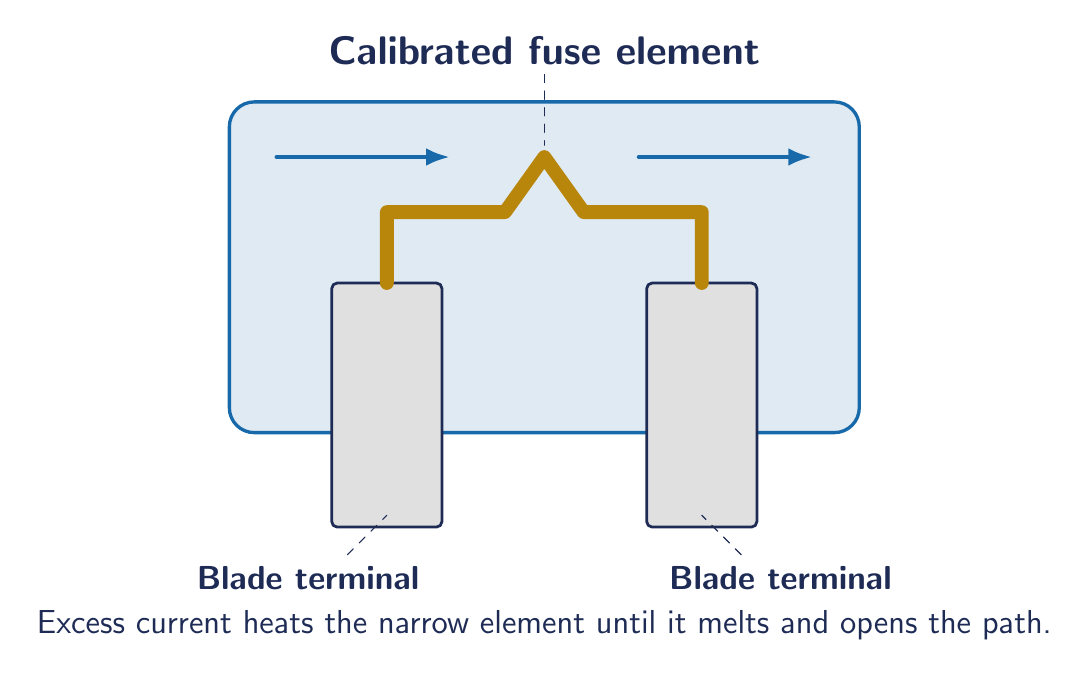
\begin{tikzpicture}[line cap=round,line join=round]
  \filldraw[fill=TEJBlue!14,draw=TEJBlue,line width=1.2pt,rounded corners=9pt]
    (1.5,1.2) rectangle (9.5,5.4);
  \filldraw[fill=black!12,draw=TEJNavy,line width=1.0pt,rounded corners=2pt]
    (2.8,0) rectangle (4.2,3.1);
  \filldraw[fill=black!12,draw=TEJNavy,line width=1.0pt,rounded corners=2pt]
    (6.8,0) rectangle (8.2,3.1);
  \draw[TEJGold,line width=5pt]
    (3.5,3.1) -- (3.5,4.0) -- (5.0,4.0) -- (5.5,4.7) -- (6.0,4.0) -- (7.5,4.0) -- (7.5,3.1);
  \node[font=\bfseries\Large,text=TEJNavy] at (5.5,6.05) {Calibrated fuse element};
  \draw[TEJNavy,dashed] (5.5,5.75) -- (5.5,4.85);
  \node[font=\bfseries\large,text=TEJNavy] at (2.5,-0.65) {Blade terminal};
  \node[font=\bfseries\large,text=TEJNavy] at (8.5,-0.65) {Blade terminal};
  \draw[TEJNavy,dashed] (3.0,-0.35) -- (3.5,0.15);
  \draw[TEJNavy,dashed] (8.0,-0.35) -- (7.5,0.15);
  \draw[-{Latex[length=3mm]},TEJBlue,line width=1.5pt] (2.1,4.7) -- (4.3,4.7);
  \draw[-{Latex[length=3mm]},TEJBlue,line width=1.5pt] (6.7,4.7) -- (8.9,4.7);
  \node[font=\large,text=TEJNavy,align=center] at (5.5,-1.25)
    {Excess current heats the narrow element until it melts and opens the path.};
\end{tikzpicture}
\end{document}
